\documentclass{article}

\usepackage{graphicx}
\usepackage{tikz}
\usepackage{tikzsymbols}
\usetikzlibrary{calc,patterns,shapes.geometric}
\pagestyle{empty}
\usepackage[margin=0pt]{geometry}
\geometry{papersize={14in,12in}}

\def\centerarc[#1](#2)(#3:#4:#5){\draw[#1] ($(#2)+({#5*cos(#3)},{#5*sin(#3)})$) arc (#3:#4:#5);}

\begin{document}
	\begin{figure}
		\centering
		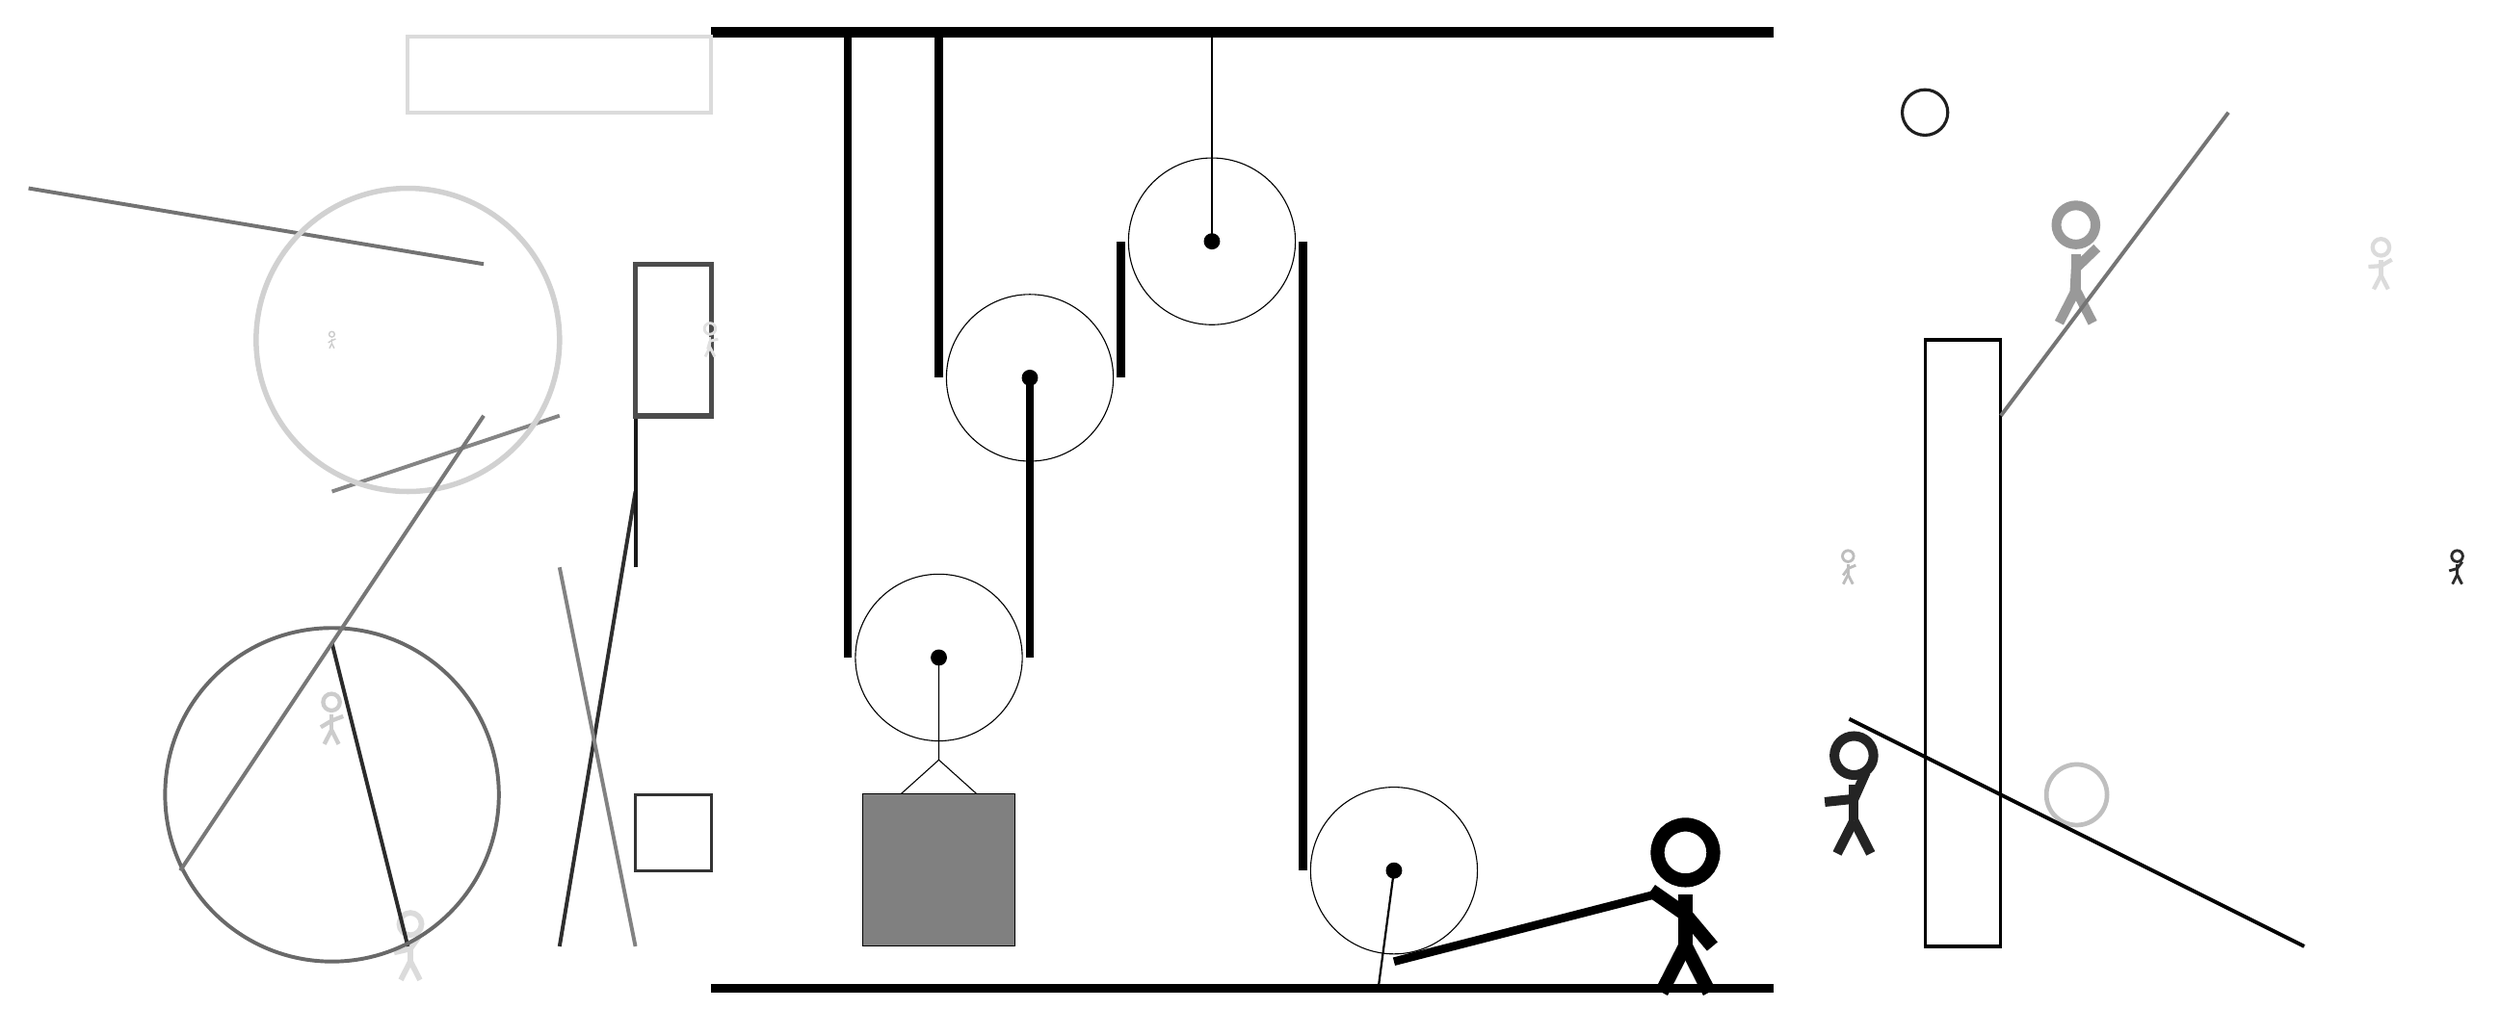
\begin{tikzpicture}
			%%%%% START %%%%%
			
			\draw[fill=black] (-2, 9) rectangle (12, 9.125);
			
			\draw (1, 0.81) circle (1.1);
			\draw[fill=black] (1, 0.81) circle (0.1);
			
			\draw[line width=0.5mm, color=black!82](-3, 3) -- (-4, -3);
			
			\draw [line width=0.4mm, color=black!88](14, 8) circle (0.3);
			\draw[line width=0.5mm, color=black!90](-3, 2) -- (-3, 6);
			\node[line width=0.6mm, color=black!20] at (-7, 5) {\Strichmaxerl[1][31][22]};
			
			\draw[line width=0.5mm, color=black!49](-4, 2) -- (-3, -3);
			
			\draw[line width=0.5mm, color=black!48](-4, 4) -- (-7, 3);
			
			\node[line width=0.5mm, color=black!14] at (-6, -3) {\Strichmaxerl[4][13][55]};
			\node[line width=0.4mm, color=black!14] at (20, 6) {\Strichmaxerl[3][4][30]};
			\draw[line width=0.4mm, color=black!80] (-3, -1) rectangle (-2, -2);
			\draw[line width=0.7mm, color=black!70] (-2, 6) rectangle (-3, 4);
			\draw [line width=0.6mm, color=black!25](16, -1) circle (0.4);
			\node[line width=0.3mm, color=black!20] at (-7, 0) {\Strichmaxerl[3][31][21]};
			\node[line width=0.7mm, color=black!12] at (-2, 5) {\Strichmaxerl[2][74][14]};
			
			\node[line width=0.5mm, color=black!26] at (13, 2) {\Strichmaxerl[2][54][23]};
			\draw[line width=0.5mm, color=black!55](-5, 6) -- (-11, 7);
			\node[line width=0.2mm, color=black!40] at (16, 6) {\Strichmaxerl[7][87][44]};
			
			\node[line width=0.3mm, color=black!86] at (13, -1) {\Strichmaxerl[7][6][66]};
			
			\draw[line width=0.5mm, color=black!83](-6, -3) -- (-7, 1);
			\draw[line width=0.4mm, color=black!100] (14, 5) rectangle (15, -3);
			\draw [line width=0.7mm, color=black!18](-6, 5) circle (2.0);
			\draw[line width=0.5mm, color=black!99](13, 0) -- (19, -3);
			\draw [line width=0.5mm, color=black!59](-7, -1) circle (2.2);
			\draw[line width=0.5mm, color=black!14] (-2, 9) rectangle (-6, 8);
			\draw[line width=0.5mm, color=black!54](15, 4) -- (18, 8);
			\node[line width=0.3mm, color=black!83] at (21, 2) {\Strichmaxerl[2][16][53]};
			
			\draw[line width=0.5mm, color=black!53](-5, 4) -- (-9, -2);
			
			\draw (2.2, 4.5) circle (1.1);
			\draw[fill=black] (2.2, 4.5) circle (0.1);
			
			\draw (4.6, 6.3) circle (1.1);
			\draw[fill=black] (4.6, 6.3) circle (0.1);
			\draw[thick] (4.6, 6.3) -- (4.6, 9);
			
			\draw (7.0, -2) circle (1.1);
			\draw[fill=black] (7.0, -2) circle (0.1);
			\draw[thick] (7.0, -2) -- (6.8, -3.5);
			
			\draw (1, 0.81) -- (1, -0.54) -- (0.5, -0.99) -- (1.5, -0.99) -- (1, -0.54);
			\draw[fill=black!50] (0, -0.99) rectangle (2, -2.99);
			\draw[line width=1.1mm] (-0.2, 9) -- (-0.2, 0.81);
			\centerarc[line width=1.1mm](1, 0.81)(180:360:1.2000000000000002);
			\draw[line width=1.1mm](2.2, 0.81) -- (2.2, 4.5);
			\draw[line width=1.1mm] (1.0, 9) -- (1.0, 4.5);
			\centerarc[line width=1.1mm](2.2, 4.5)(180:360:1.2000000000000002);
			\draw[line width=1.1mm](3.4, 4.5) -- (3.4, 6.3);
			\centerarc[line width=1.1mm](4.6, 6.3)(0:180:1.2000000000000002);
			\draw[line width=1.1mm] (5.8, 6.3) -- (5.8, -2);
			\centerarc[line width=1.1mm](7.0, -2)(0:90:-1.2000000000000002);
			\draw[line width=1.1mm](7.0, -3.2) -- (10.5, -2.3);
			
			\node at (10.8, -2.5) {\Strichmaxerl[10][-35][-50]};
			
			\draw[fill=black] (-2, -3.5) rectangle (12, -3.6);
			
			%%%%% END %%%%%
		\end{tikzpicture}
	\end{figure}	
\end{document}